\subsection{K-means}
K-means is used to group the data set into categories depending on their location in the x-dimensional space determined by the amount of features representing one of them.
The center of these clusters are then computed and identified as a specific category.
Using these centres, a unknown element can then be categorized depending on which cluster is the closest.

To find the number of clusters best representing the data set, then the within-group heterogeneity and homogeneity was computed for various K's as seen on figure \ref{fig:elbow_point}.
The elbow point can from here be determined to be at K of 1300 where it has 73.6\% homogeneity.

% It is also shown that normalizing the data or using a filter doesn't improve the performance. It actually hurts the performance. 

% k_means_elbow.R
\begin{figure}[H]
\centering
\begin{subfigure}{0.70\textwidth}
\centering
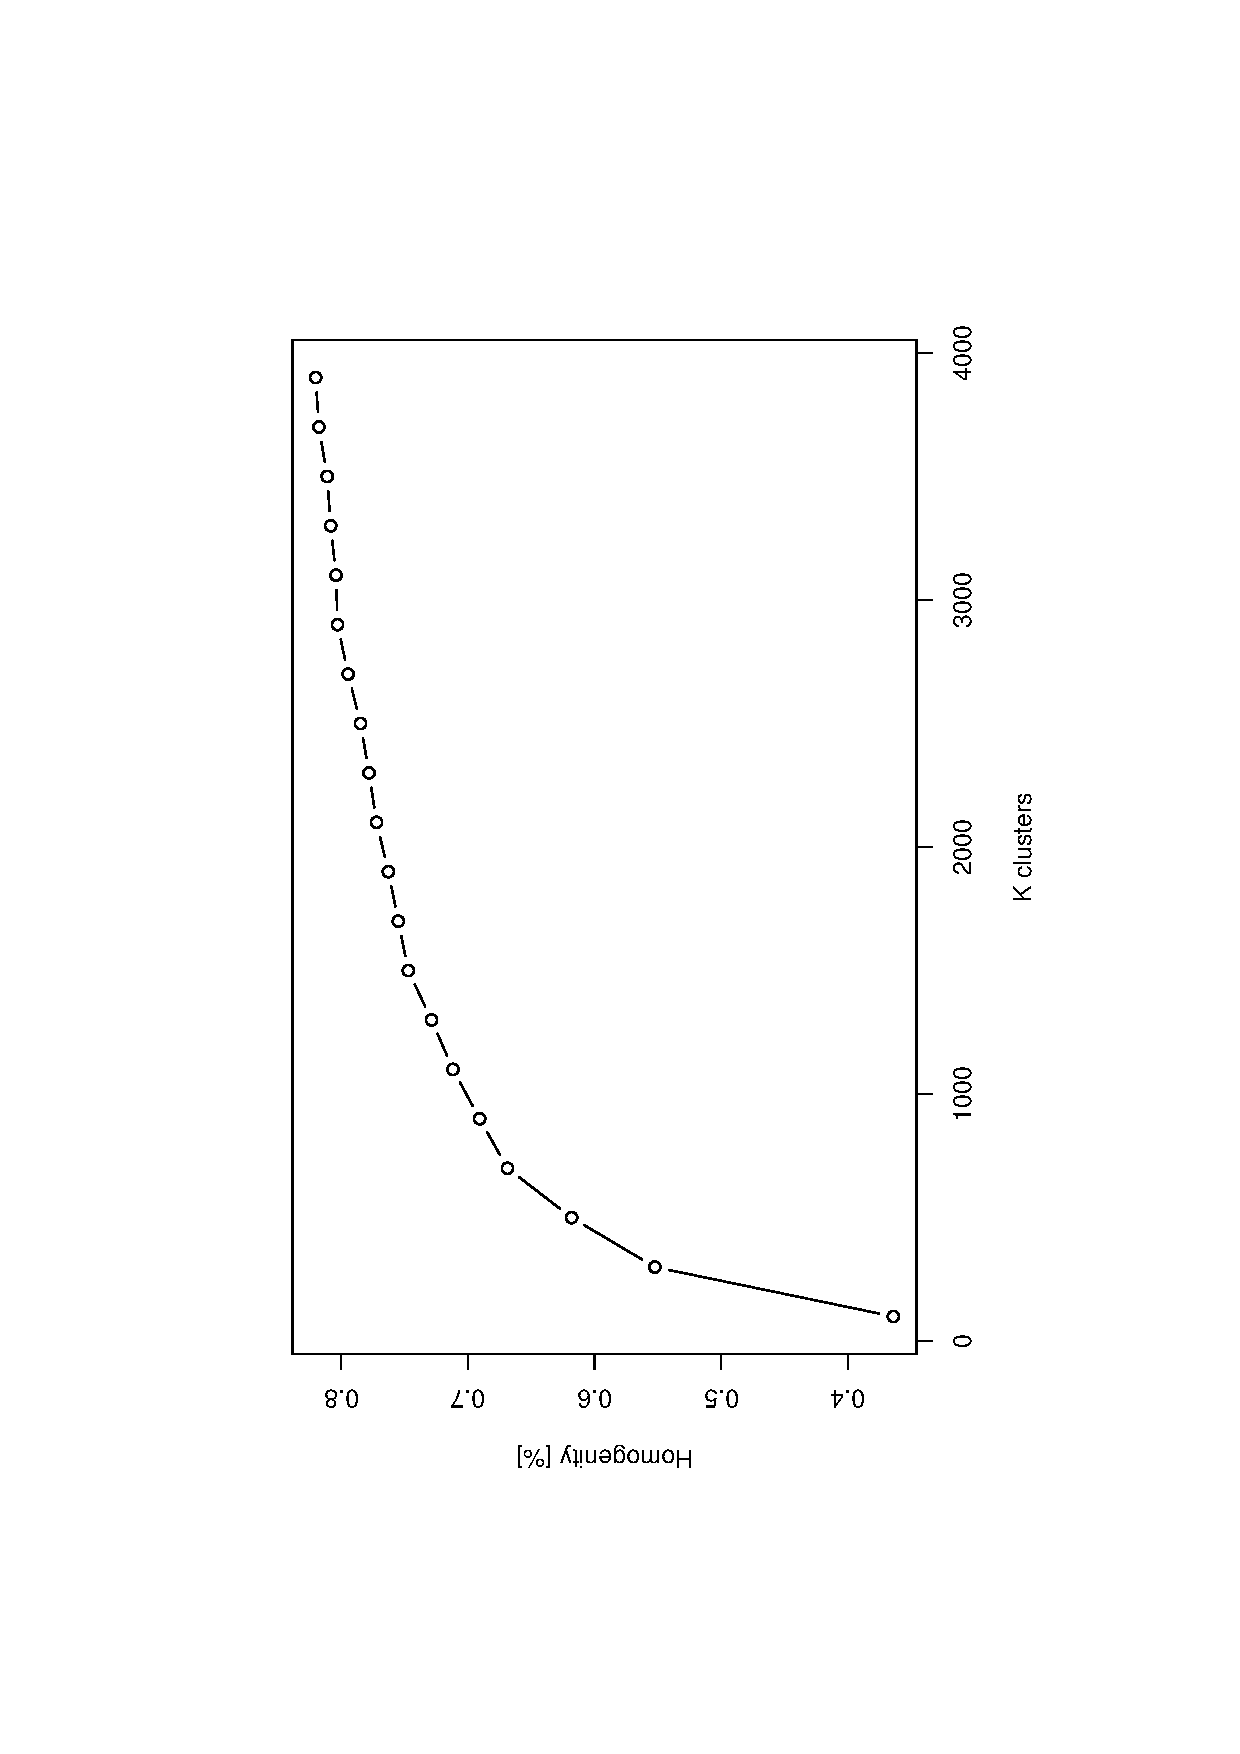
\includegraphics[width=\textwidth]{graphics/homogenity}
\caption{homogeneity}
\label{fig:homogeneity_kmean}
\end{subfigure}\\[-1cm]
\begin{subfigure}{0.70\textwidth}
\centering
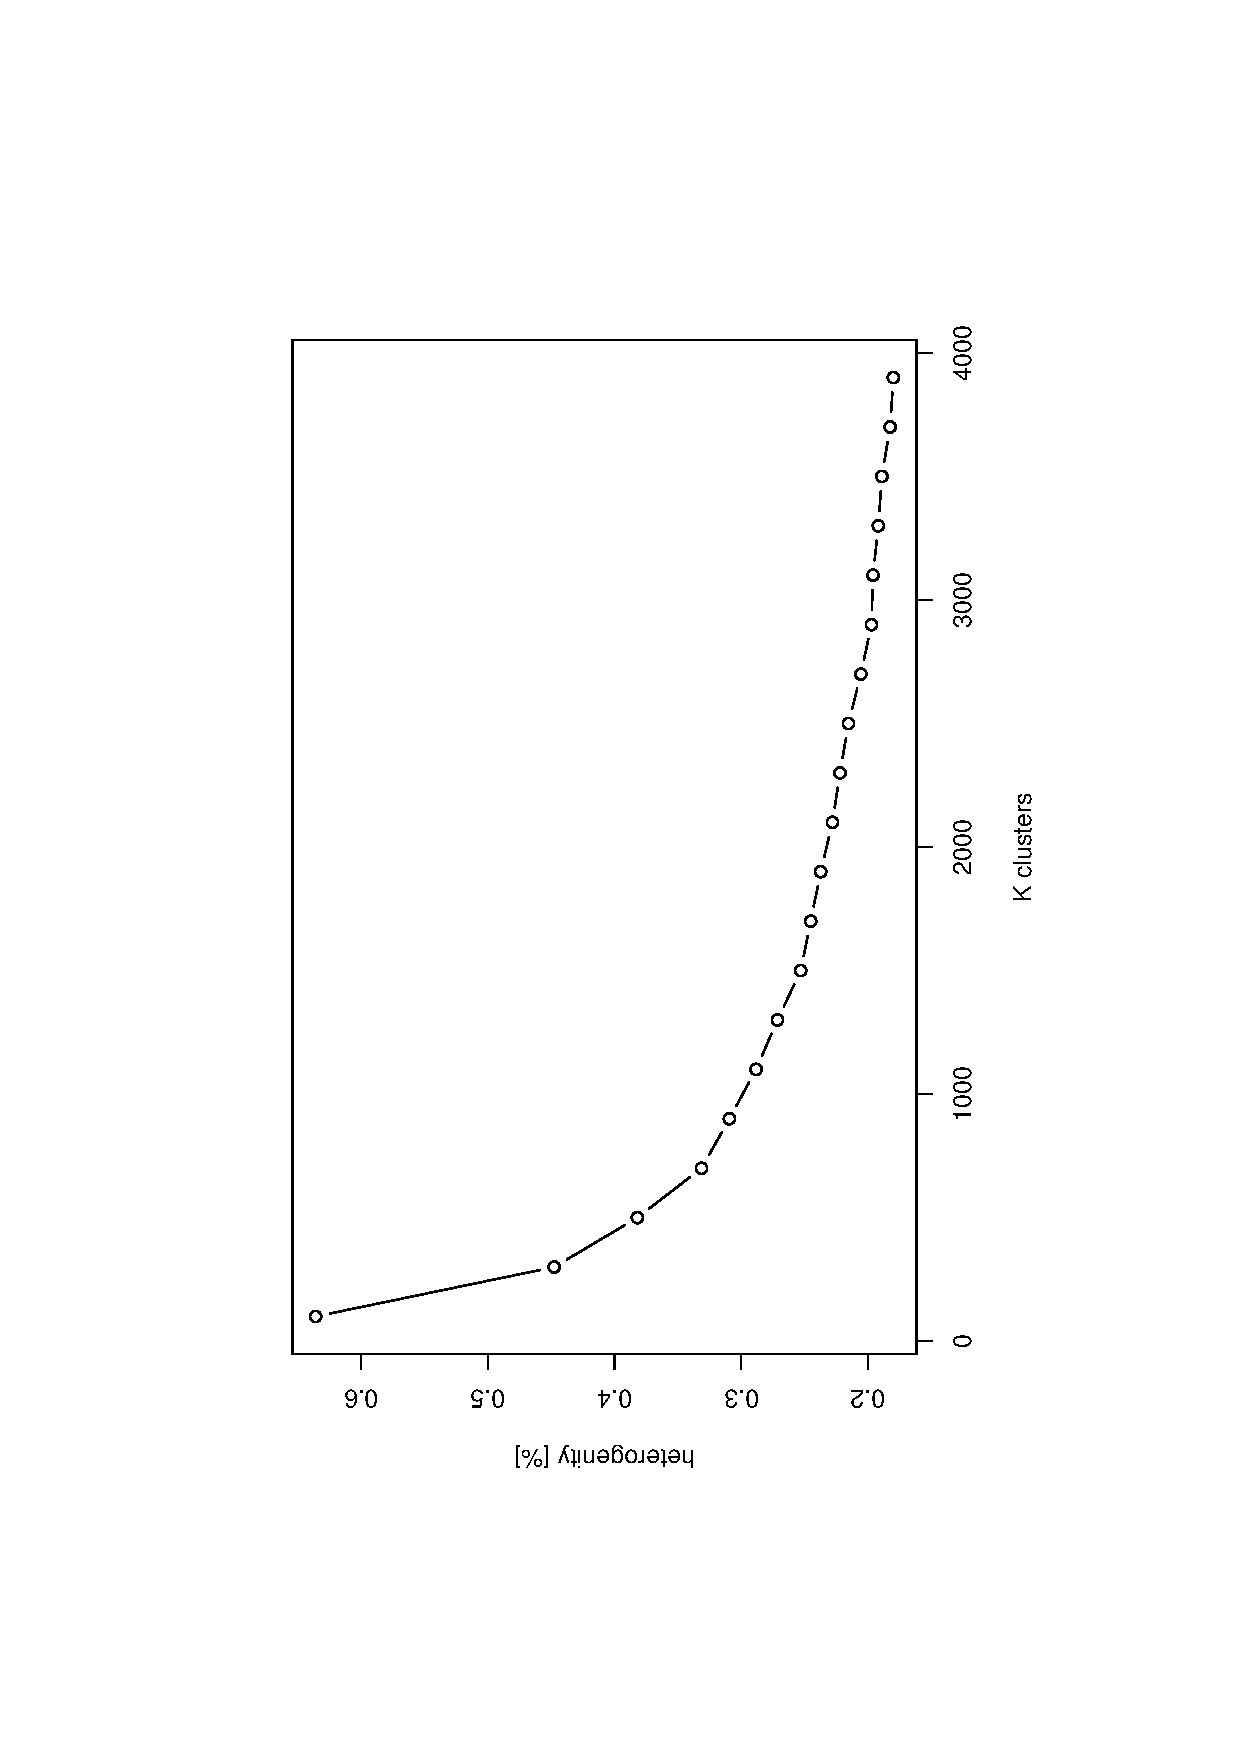
\includegraphics[width=\textwidth]{graphics/heterogenity}
\caption{heterogeneity}
\label{fig:heterogeneity_kmean}
\end{subfigure}
\caption[K means elbow point]{homogeneity and heterogeneity of the data set.}
\label{fig:elbow_point}
\end{figure}


\begin{table}[H]
\centering
%# kmean = 1500
%# k_knn = 10
%# k_mean = 10
%# kmean_iterations = 500
%# Time taken to prep kmean: 747.229999999996
%# Time taken to run kmean classification: 42.1600000000035
%# Success for kmean: 0.54275
%# Time taken to prep norm kmean: 802.549999999996
%# Time taken to run norm kmean classification: 44.4400000000023
%# Success for norm kmean: 0.63125
%# Time taken to run raw knn classification: 1878.1
%# Success for raw knn: 0.73625

% \begin{tabular}{|l|p{2cm}|p{2cm}|p{2cm}|}\hline
% Criteria              & None   & K-mean & Normalized K-mean \\ \hline
% Pre-Processing Time*  & 0s     & 12m27s & 13m23s            \\ \hline
% Classification Time** & 31m18s & 42.2s  & 44.4s             \\ \hline
% Success Rate**        & 73.6\% & 54.3\% & 63.1\%            \\ \hline
% \multicolumn{4}{|l|}{* of 60,000 elements} \\ 
% \multicolumn{4}{|l|}{** of 4,000 elements} \\ \hline
% \end{tabular}

\begin{tabular}{|l|p{2cm}|p{2cm}|p{2cm}|}\hline
Criteria              & None   & K-mean & Normalized K-mean \\ \hline
Pre-Processing Time*  & 0s     & 14m3.3s & 15m7.7s            \\ \hline
Classification Time** & 18m1.7s & 43.5s  & 39.6s             \\ \hline
Success Rate**        & 73.7\% & 54.1\% & 60.4\%            \\ \hline
\multicolumn{4}{|l|}{* of 60,000 elements} \\ 
\multicolumn{4}{|l|}{** of 4,000 elements} \\ \hline
\end{tabular}
\caption{Processing time comparison of running K-NN on K-mean data, normalized + k-mean data and raw data. K-mean makes 1300 clusters and max 500 iterations, the K-NN algorithm is applied with k = 10.}
\label{tab:processingtime_kmean_vs_raw_knn}
\end{table}